Most of the entities in the \SOP{} domain have been identified by looking for nouns in our use cases, revision being the exception.
The domain model (\ref{fig:domain-model}) contains the core entities of the \SOP{} system, and the transition to runtime entities (as seen on figure \ref{fig:design-class_diagram} on page \pageref{fig:design-class_diagram}) is obvious, except perhaps for the application of the composite pattern.
Notably, the \emph{Content} attribute of \emph{Document} is actually a \emph{Revision} in 
its own right. Only it denotes the current version of the document's contents, while the relation to the \emph{Revision} entity forms a history for the document.
\begin{figure}[hbt]
	\centering
	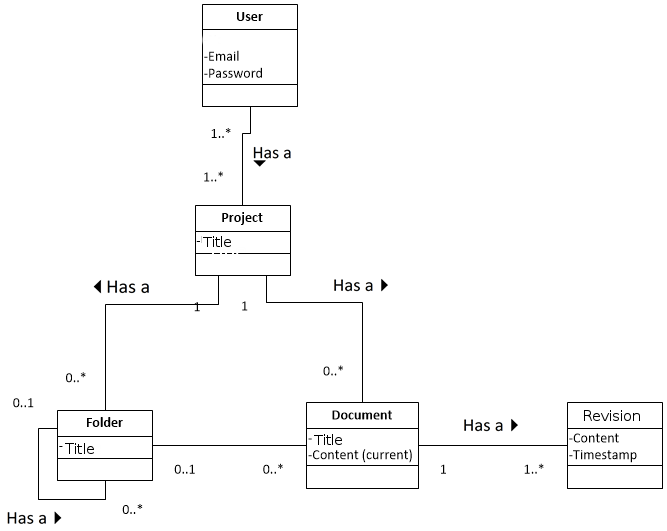
\includegraphics[width=1\textwidth]{Software_analysis/graphics/Domain_model.png}
	\caption{Domain model}
	\label{fig:domain-model}
\end{figure}
	
